In \cite{Paper2} they proposed a dynamic model for parallel H.264/AVC video encoding on hybrid GPU+CPU. First they analysed the dependencies of the encoding process of H.264/AVC. For their model to work they needed concrete information on every part of the algorithm itself and its possibility to be parallelised. These dependencies analysis showed, that parallel processing can only be considered within the scope of a single frame. Inter-prediction usually can not start before updating the list of referenced frames. The deblocking-filter for instance can not be applied on two different regions of each slice, because it has intra-frame dependencies, one point that was improved in H.265. \\
The conclusion of the analyses however indicates, that the best possibilities to process H.264 in parallel are the interpolation and the ME. Motion estimation is like already mentioned the most compute intense part of the algorithm anyway and also the main approach of the other papers reviewed in this article. Interpolation however is also interesting, because GPUs are mostly equipped with an interpolation unit.\\

\begin{figure}[H]

\begin{tikzpicture}
[
    pie chart,
    slice type={sub}{blu},
    slice type={dbl}{rosso},
    slice type={int}{giallo},
    slice type={mctq}{viola},
    slice type={fme}{verde},
    pie values/.style={font={\small}},
    scale=1.7
]
	\pie{\hypertarget{pie}{CPU}}{32/sub,2/dbl,4/int,2/mctq,60/fme}
	\pie[shift={(2.2cm,0cm)}]{\hypertarget{pie}{GPU}}{15/sub,5/dbl,4/int,1/mctq,75/fme}

    \legend[shift={(0 cm,-1 cm)}]{{SUB}/sub, {DBL}/dbl, {INT}/int}
	\legend[shift={(1 cm,-1 cm)}]{{MC\_TQ}/mctq, {FME}/fme}

\end{tikzpicture}
\caption{\label{dynamic_cpu_gpu}{\it Breakdown of the H.264/AVC interprediction-loop processing time measured by \cite{Paper2}; (FME: full-
pixel ME; SUB: sub-pixel ME; INT: interpolation; DBL: deblocking filter; MC TQ: di-
rect transform, quantization, dequantization and inverse transform) (data taken from \cite{Paper2})}}
\end{figure}

Figure \ref{dynamic_cpu_gpu} represents a breakdown of the H.264/AVC processing time for both CPU and GPU implementations, regarding the several encoding modules. These results were obtained by measuring  a highly optimized implementation on an Intel Core i7 CPU and on an NVIDIA GeForce GTX 580 GPU. However, the author doesn't really say which algorithm was used and what optimizations were done. But for the study the breakdown was used to determine the importance of each part of the codec algorithm. It can clearly be seen, that ME is the dominant module with 60\% on the CPU and 75\% on the GPU.

Because the heterogeneous structure of the H.264/AVC encoder includes modules with very different characteristics regarding the data dependencies and parallelization potential the authors analysed the possibility of minimizing the encoding time by efficiently distributing the several tasks on the CPU and on the GPU.\\

They created an algorithm which evaluates the performance of the GPU and CPU for certain parts of the encoding algorithm at runtime. That means that they chose a dynamic approach to evaluate the performance and change the amount of work for each device for each step of the algorithm during runtime. The performance is always evaluated for the previous encoded frame. This approach has of course the negative effect of having a lot of overhead for measuring the time and evaluating the best results. It also means that both devices are usually fully occupied by the encoding algorithm and run certain parts of it in parallel on both CPU and GPU. \\
To undertake this approach they created a dynamic load distribution model shown in figure \ref{dynamic_model} for tracking the individual execution times of the different parts of the H.264 algorithms on both CPU and GPU and distributing the task to the according devices.\\
For the compute intensive parts of the algorithm they measured in their breakdown (\ref{dynamic_cpu_gpu}) and that can be parallelized, their load distribution model splits the work between CPU and GPU. That means for instance that 40\% of the ME of a frame is processed on a CPU and 60\% on a GPU. Furthermore it has to be noticed that the author doesn't mention how the MVs are managed that get lost when a frame is divided between the devices.

\begin{figure*}[ht]
\centerline{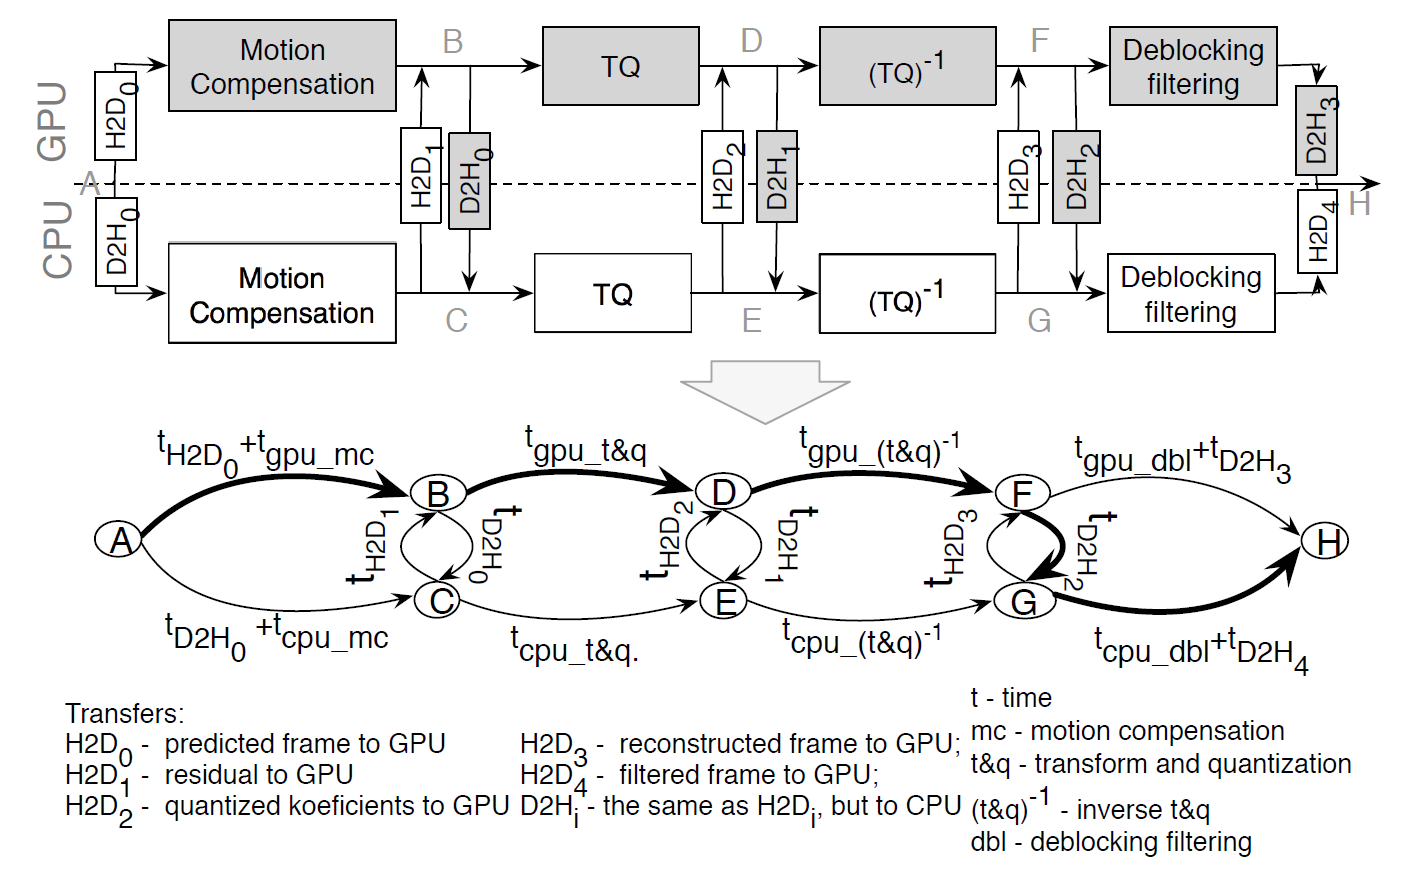
\includegraphics[scale=0.4]{pics/dynamic_model}} % The bounding box is set manually in this example. Useful for some .pdf figures.
\caption{\label{dynamic_model}{\it Construction of weighted DAG from the data-flow diagram of H.264/AVC and
a possible minimal path (represented in bold) (taken from \cite{Paper2})}}
\end{figure*} % [width=5in,bb= 36 253 574 500]

The load distribution model is characterized by its synchronization parts (upper part of figure \ref{dynamic_model}). As mentioned each step will be measured and shared with the other device to evaluate the distribution of tasks for the next frame. By doing so a weighted directed acyclic graph (DAG) will be obtained  (lower part of figure \ref{dynamic_model}). The bold path shows the possible minimal path of the encoding time for the previous frame.\\